\section{Общая методология}
\label{method}

\subsection{Требование 1}
\label{task1}

Формулировка требования: <<Отсутствуют вложенные области, т.е. все области односвязны>>.

Многосвязная область состоит из внешней границы и произвольного числа внутренних границ, заданных многоугольниками. Задача снижения порядка связности области сводится к выбору соединений точек различных границ таким образом, чтобы все они оказались связаны. В простейшем случае с одной внутренней границей подойдет любой отрезок, один из концов которого принадлежит множеству вершин внешней границы, а другой --- внутренней, и который не имеет с границами других общих точек. В случае трехсвязной области (с двумя внутренними границами) можно также соединить внутренние границы, а затем одну из них --- со внешней.

Чтобы найти требуемые соединения, преобразуем объектную модель карты следующим образом. Поставим в соответствие каждому многоугольнику, включая внешнюю границу, вершину графа и сделаем полученный граф полным. В полученной графовой модели ребра соответствуют соединениям между многоугольниками. В качестве весов присвоим им длины кратчайших соединений между соответствующими многоугольниками. Далее, нужно исключить из модели недопустимые соединения --- такие, которые имеют более двух общих точек с многоугольниками. Для этого будем проверять соединение на пересечение со всеми сторонами многоугольников в рассматриваемой области. Наконец, к полученному графу применим алгоритм Прима \cite{prim_shortest_1957} для выделения минимального остовного дерева.

\begin{figure}[h]
    \centering
    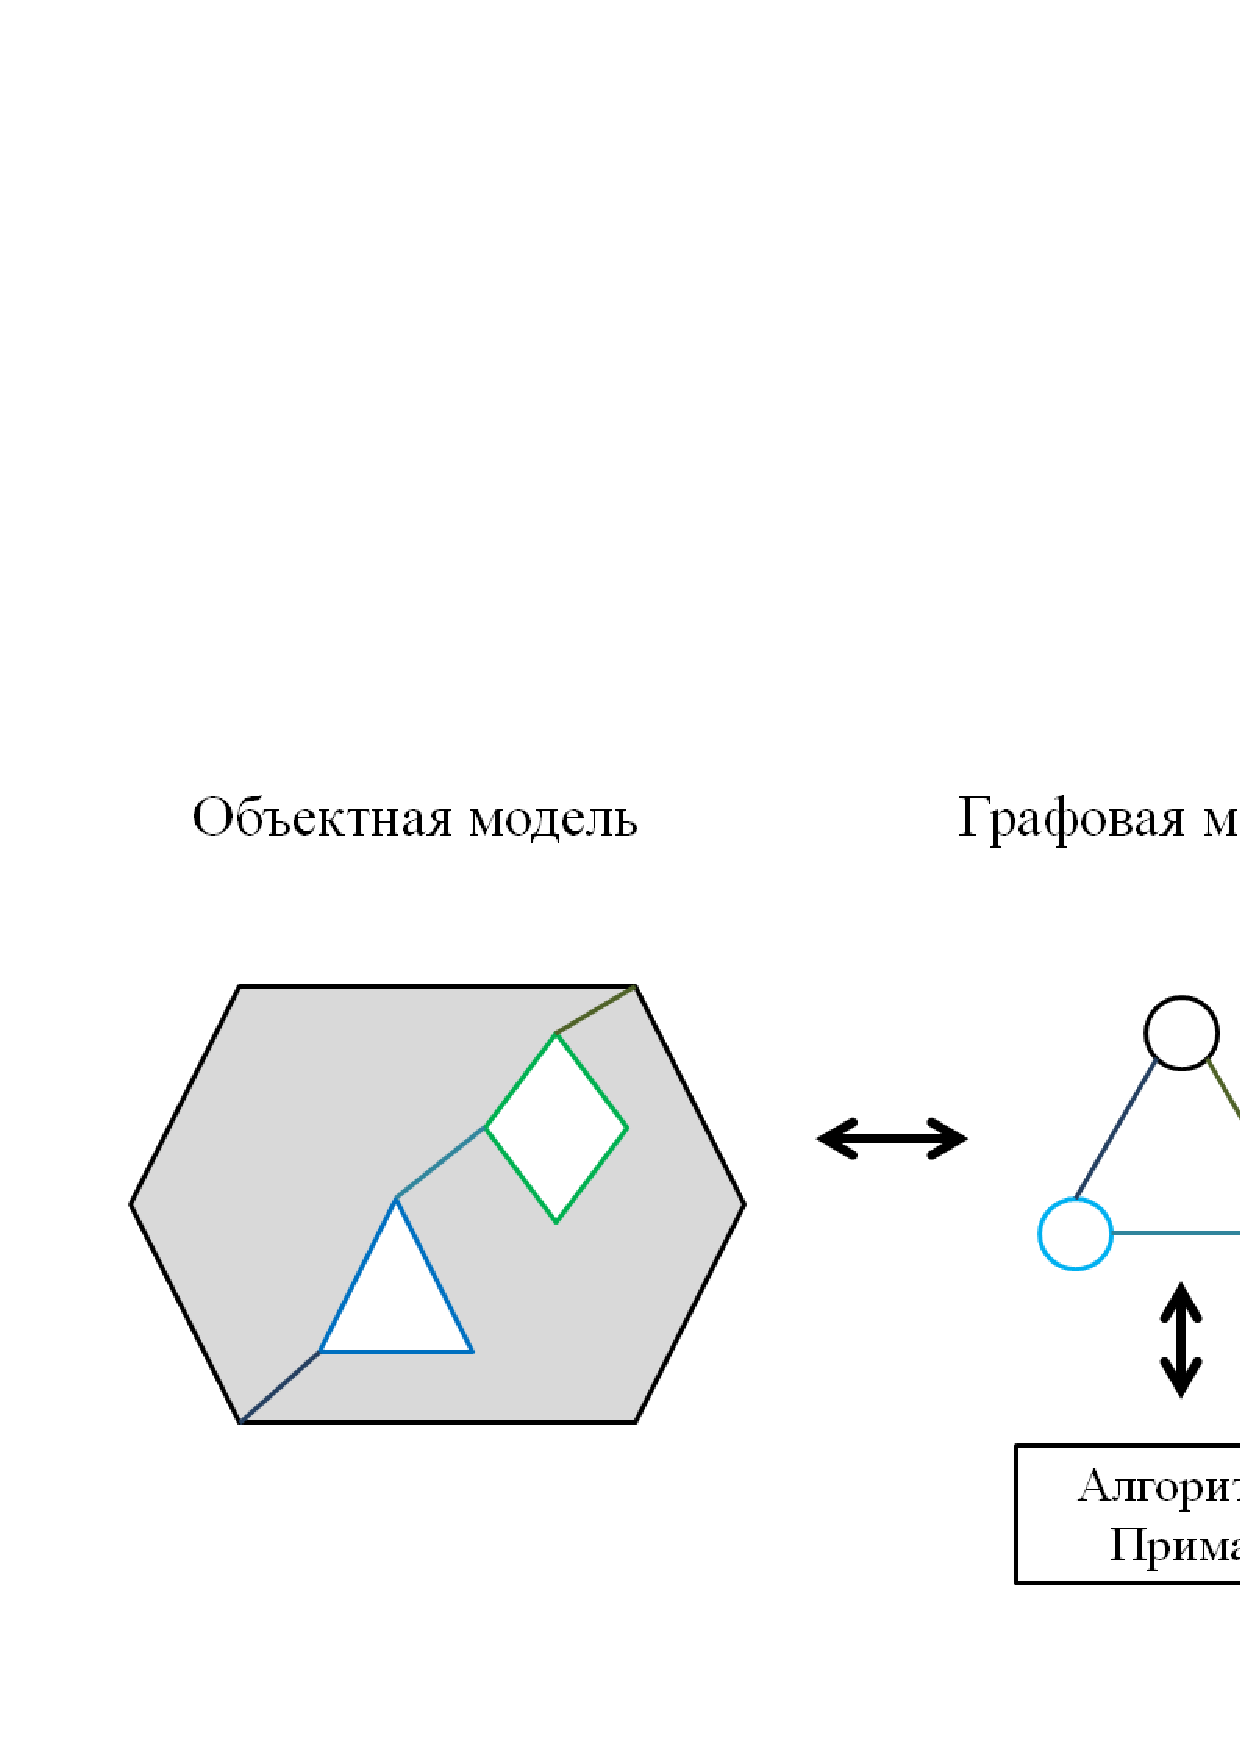
\includegraphics[width=1\textwidth]{Prim.png}
    \caption{Использование алгоритма Прима для удовлетворения требованию 1}
    \label{fig:prim}
\end{figure}

Восстановление объектной модели из графовой происходит следующим образом. На внешней границе произвольно выбирается начальная точка. Если с ней не связано ни одно из соединений в графовой модели, происходит переход к следующей вершине в том же многоугольнике; в противном случае эта вершина сохраняется в памяти, а следующей выбирается точка, находящаяся на другом конце найденного соединения, для которой та же процедура повторяется рекурсивно. Когда процесс возвращается в исходную точку, он возвращается по тому же соединению к предыдущему многоугольнику. Алгоритм завершает работу, когда возвращаться становится некуда. В результате вместо многосвязной области получается односвязная, в которой соединения становятся вырожденными туннелями.

\subsection{Требование 2}
\label{task2}

Формулировка требования: <<Число точек, задающих границу каждой области, не превышает заданной константы N>>. На данном этапе все области уже односвязны.

\begin{figure}[h]
    \centering
    \includegraphics[width=0.6\textwidth]{split.png}
    \caption{Пример разбиения пятиугольника при максимальном количестве вершин N=4: $ABCDE = ABC \cup ACDE$}
\end{figure}

Рассмотрим вначале область, задаваемую выпуклым многоугольником с более чем N вершинами. Из определения выпуклости очевидно, что ее можно разделить в произвольном отношении, т.к. любая линия, соединяющая несмежные точки, будет лежать внутри области. С учетом требования 3 следует выбрать кратчайшую линию, разделяющую многоугольник таким образом, чтобы в одной из полученных частей было ровно N вершин. Если во второй части их больше N, повторяем ту же процедуру для нее рекурсивно.

Отметим, что при разбиении выпуклого многоугольника получаются также выпуклые многоугольники, поскольку все вершины полученных многоугольников лежат по одну и ту же сторону от новой грани.

Рассмотрим теперь невыпуклые многоугольники. Согласно \cite{de_berg_chapter_2000}, любой многоугольник можно разбить на смежные треугольники. Очевидно, эти треугольники можно объединять по смежным сторонам, получая таким образом разбивку на части с произвольным количеством вершин. Следовательно, существует и такая разбивка, при которой одна из частей имеет ровно N вершин. Значит, описанный алгоритм можно распространить и на невыпуклые области.

\subsection{Требование 3}
\label{}

Формулировка требования: <<Количество добавочных соединений и их длины минимальны>>. В процессе разработки к этому условию было добавлено важное уточнение: если минимизация обоих параметров одновременно невозможна или невыполнима за полиномиальное время, приоритет имеет количество соединений.

Докажем, что после выполнения описанных выше шагов алгоритма это условие уже выполнено.

Вначале рассмотрим добавочные соединения, образовавшиеся в процессе упрощения топологии. Вспомним, что эти соединения представляют собой остовное дерево в графе всевозможных соединений, причем за вес ребра в этом графе принимается длина соединения.

По свойству дерева \cite{__2010}, количество его ребер фиксировано: $B-P=1$, где $B$ — число вершин, $P$ — число рёбер графа. Следовательно, удаление любого из оставшихся соединений приведет к тому, что объект карты перестанет быть односвязным. Значит, условие минимальности количества дополнительных соединений выполняется.

Для выбора минимальных соединений из графа всех возможных соединений использовался алгоритм Прима. Из его корректности \cite{prim_shortest_1957} следует, что выбранное остовное дерево графа является минимальным. Значит, условие минимальности длин дополнительных соединений выполняется. Таким образом, требование 3 удовлетворено.

Теперь рассмотрим добавочные соединения, образовавшиеся в процессе уменьшения числа вершин.

Пусть дан многоугольник с $V$ вершинами. Тогда описанный выше алгоритм разобьет его на $M$ частей, причем $(M-1)*N < V+2*M \leq M*N$ (слагаемое $2M$ добавляется за счет того, что вершины, через которые проводится разделяющая линия, дублируются в результирующих многоугольниках). Очевидно, что при уменьшении $M$ на единицу количество вершин как минимум одного полученного после разбиения многоугольника будет превышать $M$; следовательно, условие минимальности количества дополнительных соединений выполняется.

Одновременная минимизация добавочных соединений и их длины теоретически возможна, но также требует полиномиального времени выполнения. С учетом примечания к требованию 3, решено было ограничиться результатами разработанного алгоритма, который дает оптимальное или близкое к оптимальному решение в большинстве практических случаев.

\subsection{Требование 4}
\label{}

Выполнение требования 4 очевидно, т.к. ни один из описанных выше алгоритмов не создавал новых вершин.

\subsection{Проверка допустимости соединений}
\label{}

Выше упоминалась проверка проводимых линий на допустимость, т.е. на пересечение с уже существующими линиями. Эта процедура является важной частью алгоритма, т.к. даже одно пропущенное пересечение делает непригодным весь выходной файл.

\begin{figure}[!htb]
    \centering
    \includegraphics[width=1\textwidth]{errors.png}
    \caption{Примеры недопустимых соединений (выделены красным)}
    \label{fig:errors}
\end{figure}

Единственный способ убедиться в отсутствии недопустимых соединений --- проверять каждое проводимое соединение на пересечение с каждой из линий, составляющих границы области. Для этого используется алгоритм, описанный в \cite{noauthor_introduction_2009}.

Этот алгоритм основывается на понятии ориентации. Ориентация упорядоченного списка из трех точек в зависимости от их взаимного расположения может принимать три значения:

\begin{itemize}[noitemsep]
\item по часовой
\item против часовой
\item лежат на одной прямой
\end{itemize}

Два отрезка, $(p1,q1)$ и $(p2,q2)$, пересекаются тогда и только тогда, когда верно одно из условий (см. рис. \ref{fig:segments1}):

\begin{itemize}[noitemsep]
\item $(p1, q1, p2)$ и $(p1, q1, q2)$ имеют разную ориентацию
\item $(p2, q2, p1)$ и $(p2, q2, q1)$ имеют разную ориентацию
\end{itemize}

\begin{figure}[!h]
    \centering
    \includegraphics[width=1\textwidth]{linesegments.png}
    \caption{Возможные ориентации отрезков в общем случае}
    \label{fig:segments1}
\end{figure}

Отдельно следует рассмотреть случай коллинеарных отрезков. Они пересекаются, если одновременно выполняются условия (см. рис. \ref{fig:segments2}):

\begin{itemize}[noitemsep]
\item $(p1, q1, p2)$, $(p1, q1, q2)$, $(p2, q2, p1)$, и $(p2, q2, q1)$ лежат на одной прямой
\item проекции на ось $x$ отрезков $(p1, q1)$ и $(p2, q2)$ пересекаются
\item проекции на ось $y$ отрезков $(p1, q1)$ и $(p2, q2)$ пересекаются
\end{itemize}

\begin{figure}[!h]
    \centering
    \includegraphics[width=1\textwidth]{linesegments2.png}
    \caption{Возможные ориентации коллинеарных отрезков}
    \label{fig:segments2}
\end{figure}

Докажем теперь, что проверять сами соединения на пересечения друг с другом не требуется. Для \ref{task2} утверждение очевидно: описанный алгоритм на каждом шаге исследует лишь одно соединение.

В \ref{task1} после построения полного графа допустимых соединений возникают пересечения. Однако, после выполнения алгоритма Прима они исчезнут. Почему? Предположим противное: в минимальном остовном дереве имеются ребра, соответствующие пересекающимся соединениям. Поменяем концы этих соединений таким образом, чтобы не нарушить связность графа (это всегда можно сделать, т.к. количество ребер графа не изменяется). Окажется, что длина каждого из полученных соединений меньше, чем у первоначальных. Но это противоречит корректности алгоритма Прима. Тем самым, утверждение доказано.